\chapter{Wstęp}
\label{ch:wstep}
Ostatnie lata przynoszą intensywny rozwój robotyki mobilnej. Roboty znajdują zastosowanie w coraz większej liczbie dziedzin, takich jak transport, przemysł czy wojsko. Niemniej jednak, koszt budowy robota mobilnego pozostaje wysoki, zaś znaczny ułamek kosztu urządzenia stanowią układy sensoryczne. 

Z drugiej strony zauważamy równie intensywny rozwój i rozpowszechnienie technologii bezprzewodowych takich jak Bluetooth czy Wi-Fi, które są obecnie dostępnie w niemal każdym obiekcie, zaś koszt zaimplementowania tych technologii na robocie jest relatywnie niewielki. Dlatego coraz częściej pojawiaja się pomysły, aby wykorzystać technologie bezprzewodowe do lokalizacji robotów mobilnych, szczególnie, że lokalizacja satelitarna (GPS, GLONASS) jest niedostępna w pomieszczeniach zamkiętych.

Do najpopularniejszych metod lokalizacji należą m. in:
\begin{itemize}
 \item lokalizacja w oparciu o wizualne znaczniki i system ich rozpoznawania
 \item lokalizacja na podstawie stereowizji
 \item odometria
 \item lokalizacja na podstawie odległości od znaczników (radiowych, akustycznych itp)
 \item lokalizacja w oparciu o skaner laserowy
\end{itemize}

Jedną z najpopularniejszych i najbardziej skutecznych spośród ww. metod jest lokalizacja w oparciu o skaner laserowy. Jednakże koszt takiego skanera wynosi ok. 2500 zł, podczas gdy zestaw znaczników radiowych działających w technologii Bluetooth wraz z kartą Wi-Fi / Bluetooth ze złączem PCI-E kosztuje ok. 200 zł (ceny na rok 2017 wg sklepu Kamami.pl). Ponadto, lokalizacja w oparciu o skaner laserowy posiada szereg wad, z których najpoważniejszą jest tzw. problem porwanego robota. Jeśli robot lokalizowany za pomocą skanera zostanie przeniesiony w inne miejsce, w którym skan laserowy daje podobny kontur, robot nie będzie w stanie stwierdzić, że został przeniesiony. Jest to szczególnie poważny problem dla robotów pracujących w budynkach posiadających wiele podobnych pomieszczeń. 

Biorąc pod uwagę powyższe rozważania, celem niniejszej pracy jest zbadanie przydatności znaczników radiowych wykorzystujących technologię Bluetooth w lokalizacji robota. Praca obejmuje następujące aspekty:
\begin{itemize}
 \item Analizę teoretyczną i eksperymentalną zależności siły sygnału radiowego w zależności od odległości między odbiornikiem a nadajnikiem,
 \item Przegląd możliwych technik lokalizacji z wykorzystaniem znaczników radiowych,
 \item Implementację i analizę eksperymentalną wybranych algorytmów lokalizacji,
 \item Implementację i analizę eksperymentalną systemu wspomagania lokalizacji laserowej za pomocą znaczników radiowych. 
\end{itemize}


W dalszej części rozdziału pokrótce przedstawiono lokalizację w oparciu o skaner laserowy, jej wady oraz zalety. W rozdziale drugim przedstawiono zarys teoretyczny problemu propagacji fal radiowych w pomieszczeniu, metody obliczania odległości w oparciu o siłę sygnału radiowego oraz dokonano przeglądu najpopularniejszych technologii radiowych pasma ISM. Rozdział trzeci jest poświęcony metodom lokalizacji, jakie są możliwe do zrealizowania za pomocą danych ze znaczników radiowych. W rozdziale czwartym opisano zrealizowany system lokalizacji, natomiast rozdział piąty zawiera wyniki testów i pomiarów systemu. Ostatni rozdział przedstawia interpretację i wnioski płynące z eksperymentów.  

\section{Metody lokalizacji w oparciu o odometrię i skaner laserowy}
Sensory odometryczne oraz skanery laserowe (tzw. lidary) to obecnie jedne z najpopularniejszych sensorów wykorzystywanych do lokalizowania robotów mobilnych. Poniżej przedstawiono ich charakterystykę oraz główne wady i zalety. 
\subsection{Odometria}
Odometria polega na pośrednim pomiarze położenia robota na podstawie jego przemieszczeń. Przemieszczenia są wyznaczane na podstawie pomiaru kątu obrotu kół robota za pomocą enkoderów inkrementalnych. Podstawowym elementem takiego sensora jest tarcza kodowa z podziałką w postaci kresek na przemian odbijających i nieodbijających światła (lub przepuszczających i nieprzepuszczających, rys. \ref{fig:encoder}). Tarcza obraca się razem z napędem robota, zaś podziałka jest oświetlana za pomocą diody podczerwonej. Optyczny układ odczytowy zlicza impulsy świetle które odbiły się od odbijających kresek na tarczy. Znając kinematykę robota, na podstawie zliczonych impulsów można wyznaczyć kąt o jaki obróciły się koła oraz drogę jaką robot przebył. Odometria należy do metod zliczeniowych, tzn. położenie robota jest wyznaczane poprzez zliczanie impulsów. Aby to położenie było wyznaczone dokładnie, muszą być spełnione pewne założenia:
\begin{itemize}
 \item średnice oraz rozstaw kół są znane,
 \item koła są współosiowe,
 \item styk kół z podłożem jest punktowy,
 \item nie zachodzi poślizg kół.  
\end{itemize}

Niespełnienie powyższych założeń jest podstawowym źródłem błędu pomiaru odometrii, który kumuluje się z czasem. Dlatego odometria nie sprawdza się w lokalizacji na dłuższych dystansach. Natomiast radzi sobie bardzo dobrze w pomiarze przyrostu położenia, wykorzystywanym przez algorytmy lokalizacji oparte na filtrach bayesowskich \cite{preskrypt}. Jej kolejną zaletą jest niska cena, prosta budowa i powszechna dostępność w większości dostępnych w sprzedaży platfom mobilnych.

\begin{figure}[H]
\centering
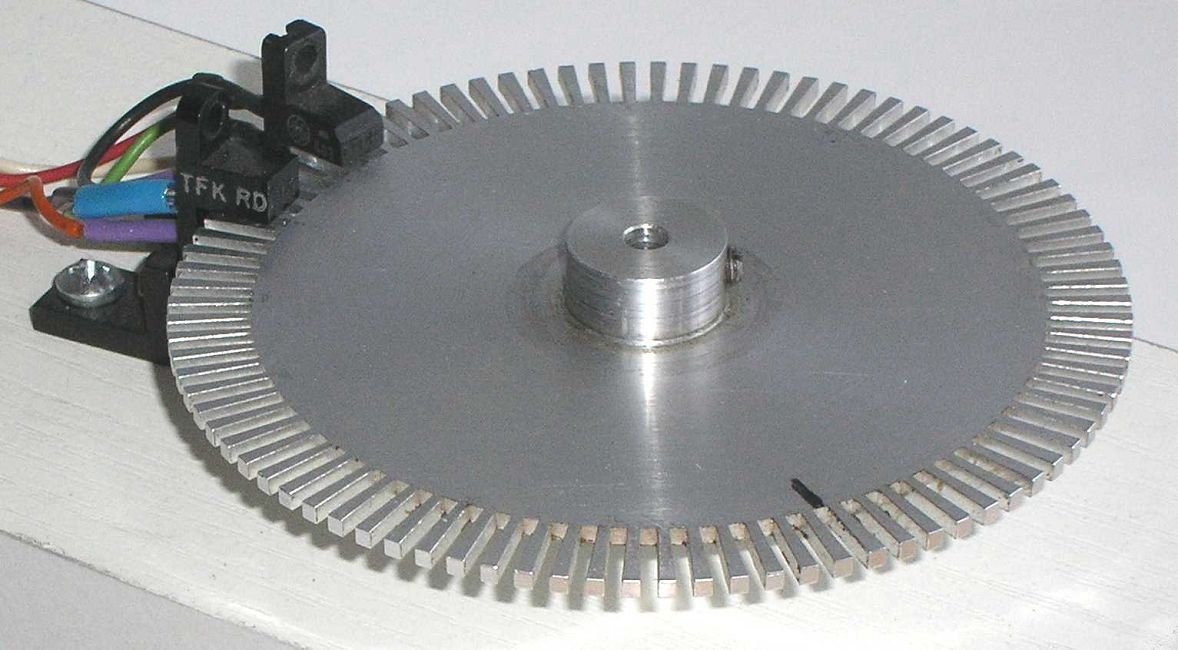
\includegraphics[width=0.7\textwidth]{img/encoder.png}
\caption{Enkoder inkrementalny wykorzystywany w odometrii}
\label{fig:encoder}
\end{figure}

\subsection{Skaner laserowy}
Współcześnie wykorzystywane dalmierze laserowe z funkcją skanowania wykorzystują metodę \textit{time of flight}, polegającą na wysłaniu impulsu świetlnego w danym kierunku i mierzeniu czasu, który upływa do powrotu impulsu odbitego od przeszkody. Na podstawie wartości tego czasu, znając prędkość światła, można wyznaczyć odległość od przeszkody. Aby osiągnąć pełny skan pomieszczenia, taki pomiar jest powtarzany w stałym interwale kątowym, np. $\Delta \phi = 0.50 \degree$ w zakresie 180 $\degree$ lub większym. Zasadę działania skanera zobrazowano na rys. \ref{fig:lidar}. Wynikiem działania skanera jest zbiór par $(r_i, \phi_i)$, określających odległosć od przeszkody i kąt skanowania. Czas wykonania pełnego skanu jest rzędu 10 ms, zaś dokładność pomiaru odległości - rzędu 10 mm.

Skany pomieszczenia w połączeniu z danymi odometrycznymi mogą zostać wykorzystane do zbudowania mapy otoczenia za pomocą algorytmu SLAM (ang. Simultaneouos Localization and Mapping, \textit{Jednoczesna Lokalizacja i Mapowanie}). Mapowanie z użyciem map SLAM polega na dopasowaniu skanu laserowego do konturu mapy i wyliczeniu translacji i rotacji pomiędzy konturem reprezentowanym przez skan laserowy, a konturem mapy, co pozwala na zlokalizowanie robota. Istnieje szereg algorytmów dopasowania skanu do mapy, opisanych szerzej w książce \cite{probabilistic_robotics}. Połączenie danych ze skanera laserowego i odometrii za pomocą filtra cząsteczkowego pozwala na bardzo dobre lokalizowanie robota, zarówno w sytuacji nieznanej mapy (za pomocą SLAM) jak i przy wykorzystaniu już posiadanej mapy.
\begin{figure}[]
\centering
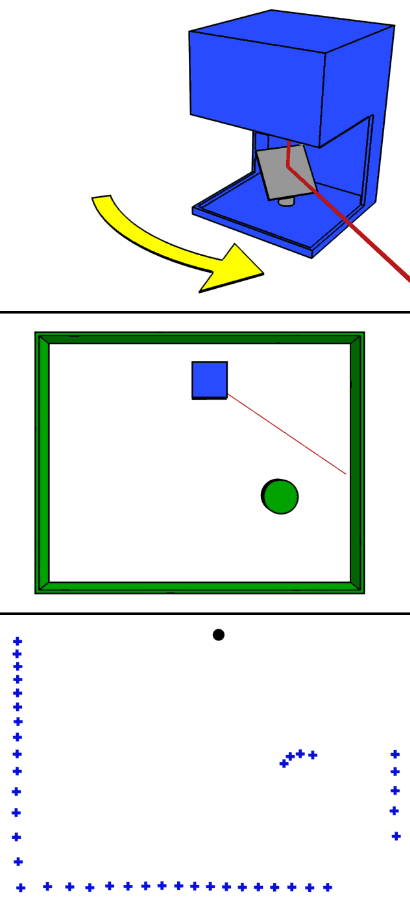
\includegraphics[width=0.5\textwidth]{img/lidar.png}
\caption{Zasada działania skanera laserowego. Od góry: 1. Kierowanie wiązki świetlnej. 2. Skanowane pomieszczenie. 3. Wynikowy zbiór punktów.}
\label{fig:lidar}
\end{figure}

\subsection{Problem porwanego robota}
Problemem porwanego robota nazywamy sytuację, w której robot lokalizowany za pomocą odometrii i/lub skanera losowego zostanie zabrany i przeniesiony do innego otoczenia. Ponieważ takiemu przemieszczeniu robota nie towarzyszy żaden obrót kół, odometria nie jest w stanie go zarejestrować. Natomiast jeśli robot zostanie przeniesiony np. z pomieszczenia o prostokątnym rozkładzie ścian do innego pomieszczenia o identycznym rozkładzie, również skaner laserowy nie będzie w stanie zdeterminować położenia robota. W wypadku lokalizacji za pomocą filtra cząsteczkowego będzie to skutkowało powstaniem dwóch (lub więcej, jeśli jest więcej podobnych pomieszczeń) skupisk cząsteczek, z których nie można jednoznacznie wybrać właściwego położenia. Podobna niejednoznaczność zachodzi często zaraz po uruchomieniu robota, kiedy jego pozycja w globalnym układzie współrzędnych pozostanie nieznana. W takiej sytuacji, dopóki robot nie wykona przejazdu, podczas którego zostaną zarejestrowane punkty charakterystyczne, nie jest możliwe określenie jego lokalizacji. 

Pomocą w takich sytuacjach może okazać się lokalizacja za pomocą znaczników radiowych. Choć jej dokładność jest niższa niż w wypadku skanera laserowego, to zgrubne wskazanie położenia na mapie może rozwiązać niejednoznaczności opisane powyżej i w rezultacie rozwiązać problem porwanego robota. 